% L2ODC3: DC3, deep constraint completion and correction.
%
% The proxy N_theta predicts the independent variables z from the parameters x;
% the equality completion phi_x(z) solves h_x([z; phi_x(z)]) = 0 for the
% dependent variables (one matrix product for affine equalities, Newton's method
% otherwise); t unrolled correction steps reduce the inequality violation along
% the equality manifold; the prediction y-hat enters the soft loss (eq. (2) of
% DC3). Gradients flow back through the corrections and, by the implicit
% function theorem (eq. (3)), through the completion. Notation follows
% docs/src/theory.md.
%
% Build: make -C docs/src/assets/diagrams/src
%   pdflatex -jobname=l2odc3--completion-correction dc3.tex          -> wide layout
%   pdflatex -jobname=l2odc3--completion-correction-compact dc3.tex  -> narrow layout
\documentclass[tikz,border=4pt]{standalone}
% Shared style of the LearningToOptimize diagrams: the palette, lane frames, cards,
% chips and glyphs of the paper-style TikZ figures (the same visual system as the
% PortfolioOpt.jl and DecisionRules.jl figures). Each figure \input's this file.
\usepackage{amsmath,amssymb,bm}
\usepackage[T1]{fontenc}
\usepackage[scaled=0.92]{helvet}
\renewcommand{\familydefault}{\sfdefault}
\usetikzlibrary{arrows.meta,shapes.geometric,shapes.symbols,calc,positioning,decorations.pathreplacing}

\definecolor{dTeal}{HTML}{1A9AA0}
\definecolor{dTealLine}{HTML}{3FB3B8}
\definecolor{dNavy}{HTML}{3F4C8C}
\definecolor{dInk}{HTML}{1E2235}
\definecolor{dRed}{HTML}{E4573D}
\definecolor{dCoral}{HTML}{E2765A}
\definecolor{dOrange}{HTML}{F4A93B}
\definecolor{dPeach}{HTML}{FBD9AC}
\definecolor{dPanel}{HTML}{EEF0F2}
\definecolor{dGray}{HTML}{8A90A0}
\definecolor{dNode}{HTML}{14A3A8}
\definecolor{dShadow}{HTML}{D5DAE3}

% \ifcompact is true when the job name ends in "-compact" (narrow layout).
\newif\ifcompact
\ifnum\pdfmatch{-compact$}{\jobname}=1 \compacttrue\fi

\tikzset{
  >={Stealth[length=5pt,width=4pt]},
  every node/.style={text=dInk},
  title/.style={anchor=west,font=\small,inner sep=0pt},
  head/.style={font=\small\bfseries,text=dNavy},
  note/.style={font=\itshape\footnotesize,text=dNavy},
  dnote/.style={font=\itshape\footnotesize,text=dCoral},
  code/.style={font=\ttfamily\footnotesize,text=dNavy},
  store/.style={cylinder,shape border rotate=90,aspect=0.28,fill=dPeach,draw=dOrange,
                line width=0.7pt,minimum width=0.95cm,minimum height=1.2cm,font=\normalsize},
  dia/.style={diamond,fill=dOrange,draw=none,minimum size=0.9cm,inner sep=0pt,aspect=1,
              font=\normalsize},
  lnode/.style={circle,fill=dRed,draw=none,minimum size=0.66cm,inner sep=1pt,
                text=white,font=\normalsize},
  card/.style={rectangle,rounded corners=4pt,fill=white,draw=dShadow,line width=0.6pt},
  sheet/.style={rectangle,rounded corners=3pt,fill=dPanel,draw=dShadow,line width=0.6pt},
  chip/.style={rectangle,rounded corners=3pt,fill=dPanel,draw=none,font=\small,
               inner xsep=4pt,inner ysep=3pt},
  ochip/.style={chip,fill=white,draw=dGray,dashed,line width=0.6pt},
  pchip/.style={chip,fill=white,draw=dGray!70,dashed,line width=0.5pt,text=dGray},
  fwd/.style={->,dTealLine,line width=0.8pt},
  tgt/.style={->,dOrange,line width=0.9pt},
  dual/.style={->,dCoral,dashed,line width=0.9pt},
  dep/.style={->,dTealLine,line width=0.8pt},
  pdep/.style={->,dGray,dashed,line width=0.7pt},
  nn/.style={circle,minimum size=0.26cm,inner sep=0pt,draw=dInk!70,line width=0.35pt},
}

% Lane frame in the paper style: two shadow copies behind a teal rounded frame.
\newcommand{\lane}[4]{% #1 x0, #2 y0, #3 x1, #4 y1
  \foreach \o/\c in {0.16/dShadow!60,0.08/dShadow}
    \draw[\c,fill=white,rounded corners=5pt,line width=0.6pt]
      (#1+\o,#2-\o) rectangle (#3+\o,#4-\o);
  \draw[dTealLine,fill=white,rounded corners=5pt,line width=0.9pt] (#1,#2) rectangle (#3,#4);}

% Plain card frame (no shadow copies), for problems and losses.
\newcommand{\cardbox}[4]{\draw[dShadow,fill=white,rounded corners=4pt,line width=0.6pt] (#1,#2) rectangle (#3,#4);}

% Network glyph on one sheet. #1 = centre, #2 = name prefix, #3 = number of stacked
% sheets behind (0, 1 or 2).
\newcommand{\net}[3]{%
  \begin{scope}[shift={(#1)}]
    \ifnum#3>1 \node[sheet,minimum width=1.9cm,minimum height=1.8cm] at (0.30,0.22) {};\fi
    \ifnum#3>0 \node[sheet,minimum width=1.9cm,minimum height=1.8cm] at (0.15,0.11) {};\fi
    \node[sheet,minimum width=1.9cm,minimum height=1.8cm,fill=white] (#2sheet) at (0,0) {};
    \foreach \y [count=\i] in {0.36,0,-0.36} \node[nn,fill=dGray!45] (#2in\i) at (-0.64,\y) {};
    \foreach \y [count=\i] in {0.58,0.29,0,-0.29,-0.58} \node[nn,fill=dNode] (#2ha\i) at (-0.21,\y) {};
    \foreach \y [count=\i] in {0.44,0.15,-0.15,-0.44} \node[nn,fill=dNode] (#2hb\i) at (0.21,\y) {};
    \node[nn,fill=dOrange] (#2out) at (0.64,0) {};
    \foreach \a in {1,...,3} \foreach \b in {1,...,5} \draw[dGray!60,line width=0.2pt] (#2in\a) -- (#2ha\b);
    \foreach \a in {1,...,5} \foreach \b in {1,...,4} \draw[dGray!60,line width=0.2pt] (#2ha\a) -- (#2hb\b);
    \foreach \a in {1,...,4} \draw[dGray!60,line width=0.2pt] (#2hb\a) -- (#2out);
  \end{scope}}

% Jacobian mask glyph: an n x d grid with a few entries selected. #1 = centre.
\newcommand{\maskgrid}[1]{%
  \begin{scope}[shift={(#1)}]
    \foreach \i in {0,...,4} \foreach \j in {0,...,3}
      \draw[dShadow,fill=white,line width=0.4pt] (\j*0.2-0.4,-\i*0.2+0.5) rectangle ++(0.2,-0.2);
    \foreach \i/\j in {0/1,1/3,2/0,3/2,4/1}
      \draw[dOrange,fill=dOrange,line width=0.4pt] (\j*0.2-0.4,-\i*0.2+0.5) rectangle ++(0.2,-0.2);
  \end{scope}}

% Code names inside italic notes stay upright.
\newcommand{\cmd}[1]{{\upshape\ttfamily #1}}

% Software-architecture helpers: package cards, type chips and chip rows.
\tikzset{
  pkg/.style={rectangle,rounded corners=4pt,fill=white,draw=dShadow,line width=0.6pt,
              align=center,inner xsep=5pt,inner ysep=4pt,font=\footnotesize},
  pkgcore/.style={pkg,draw=dTealLine,line width=0.9pt},
  pkgplan/.style={pkg,draw=dGray,dashed,text=dGray},
  tchip/.style={chip,font=\ttfamily\footnotesize,inner xsep=3pt,inner ysep=2.5pt},
  tplan/.style={tchip,fill=white,draw=dGray,dashed,line width=0.5pt,text=dGray},
  absname/.style={anchor=west,font=\ttfamily\footnotesize,text=dNavy,inner sep=1pt},
}
% \chiprow{x}{y}{style}{A,B,C}: chips left to right from (x,y), anchored west.
\newcommand{\chiprow}[4]{%
  \coordinate (cr@next) at (#1,#2);
  \foreach \t in {#4} {%
    \node[#3,anchor=west] (cr@last) at (cr@next) {\t};
    \coordinate (cr@next) at ($(cr@last.east)+(0.12,0)$);}}


% t stacked correction steps, centred at #1
\newcommand{\unrolled}[1]{%
  \begin{scope}[shift={(#1)}]
    \node[sheet,minimum width=2.7cm,minimum height=1.25cm] at (0.30,0.20) {};
    \node[sheet,minimum width=2.7cm,minimum height=1.25cm] at (0.15,0.10) {};
    \node[sheet,minimum width=2.7cm,minimum height=1.25cm,fill=white,align=center,font=\small] (corr) at (0,0)
      {correction\\[1pt]$z\leftarrow z-\gamma\,\Delta z$};
    \node[font=\footnotesize\itshape,text=dNavy,anchor=north east] at (1.45,0.95) {$\times\,t$};
  \end{scope}}
\newcommand{\complete}{completion $\varphi_x(z)$\\[1pt]$h_x\big([z;\,\varphi_x(z)]\big)=0$}
\newcommand{\softloss}{%
  $\begin{aligned}
    \ell(\hat y)=\;& f_x(\hat y)\\
    &+\lambda_g\,\big\|\mathrm{ReLU}\big(g_x(\hat y)\big)\big\|_2^2\\
    &+\lambda_h\,\big\|h_x(\hat y)\big\|_2^2
  \end{aligned}$}
\newcommand{\ift}{$\dfrac{\partial\varphi_x(z)}{\partial z}=-\big(J^h_{:,\varphi}\big)^{-1}J^h_{:,z}$\;\;(3)}

\begin{document}
\ifcompact
% ============================ narrow (phone) layout ============================
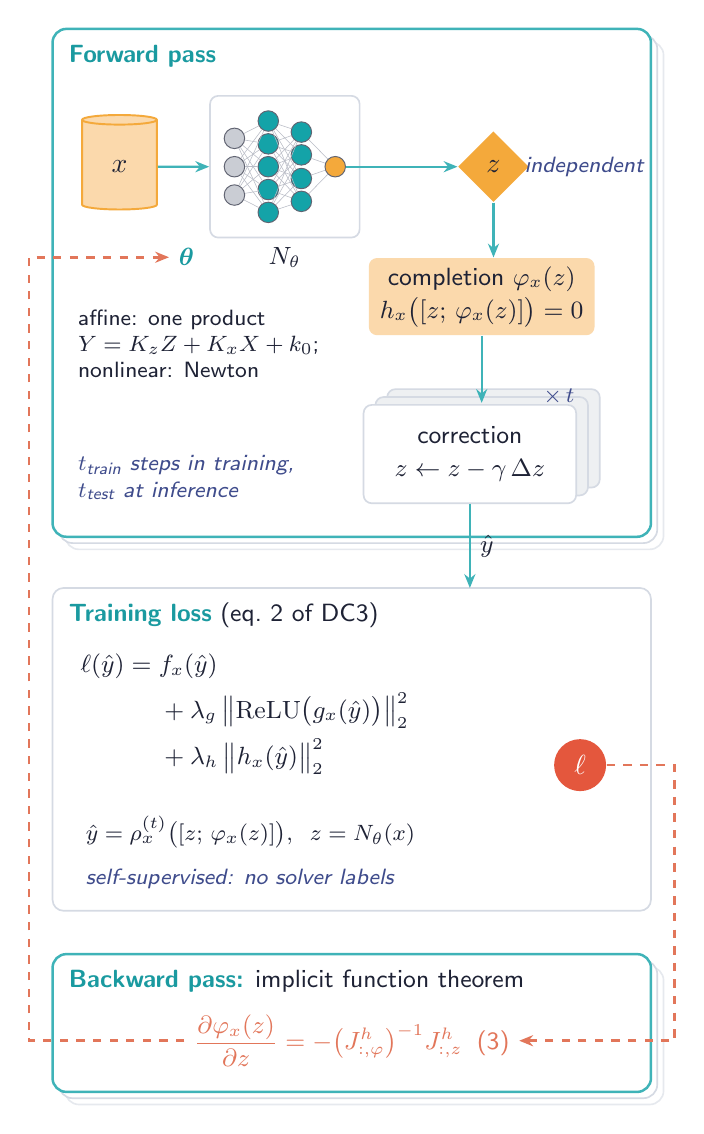
\begin{tikzpicture}
  % ---- forward ----
  \lane{0}{6.3}{7.6}{12.75}
  \node[title] at (0.2,12.4) {\textcolor{dTeal}{\bfseries Forward pass}};
  \node[store] (x) at (0.85,11.0) {$x$};
  \net{2.95,11.0}{px}{0}
  \node[font=\small] at (2.95,9.85) {$N_\theta$};
  \node[font=\small\bfseries,text=dTeal] (th) at (1.7,9.85) {$\bm\theta$};
  \draw[fwd] (x.east) -- (pxsheet.west);
  \node[dia] (z) at (5.6,11.0) {$z$};
  \draw[fwd] (pxout.east) -- (z.west);
  \node[note] at (6.75,11.0) {independent};
  \node[chip,fill=dPeach,align=center,font=\small] (cp) at (5.45,9.35) {\complete};
  \draw[fwd] (z.south) -- (5.6,9.35 |- cp.north);
  \node[font=\footnotesize,anchor=west,align=left] at (0.2,8.75) {affine: one product\\$Y=K_zZ+K_xX+k_0$;\\nonlinear: Newton};
  \unrolled{5.3,7.35}
  \draw[fwd] (cp.south) -- (5.45,8.0);
  \node[note,anchor=west,align=left] at (0.2,7.05) {$t_{\text{train}}$ steps in training,\\$t_{\text{test}}$ at inference};
  % ---- loss ----
  \cardbox{0}{1.55}{7.6}{5.65}
  \draw[fwd] (5.3,6.72) -- node[right,font=\small] {$\hat y$} (5.3,5.65);
  \node[title] at (0.2,5.3) {\textcolor{dTeal}{\bfseries Training loss} (eq.\ 2 of DC3)};
  \node[anchor=north west,font=\small,inner sep=0pt] at (0.35,4.85) {\softloss};
  \node[lnode] (l) at (6.7,3.4) {$\ell$};
  \node[font=\footnotesize,anchor=west] at (0.3,2.55) {$\hat y=\rho_x^{(t)}\big([z;\,\varphi_x(z)]\big),\;\; z=N_\theta(x)$};
  \node[note,anchor=west] at (0.3,1.95) {self-supervised: no solver labels};
  % ---- backward ----
  \lane{0}{-0.75}{7.6}{1.0}
  \node[title] at (0.2,0.65) {\textcolor{dTeal}{\bfseries Backward pass:} implicit function theorem};
  \node[font=\small,text=dCoral] (ad) at (3.8,-0.1) {\ift};
  \draw[dual] (l.east) -- (7.9,3.4) -- (7.9,-0.1) -- (ad.east);
  \draw[dual] (ad.west) -- (-0.3,-0.1) -- (-0.3,9.85) -- (th.west);
\end{tikzpicture}
\else
% =============================== wide layout ===================================
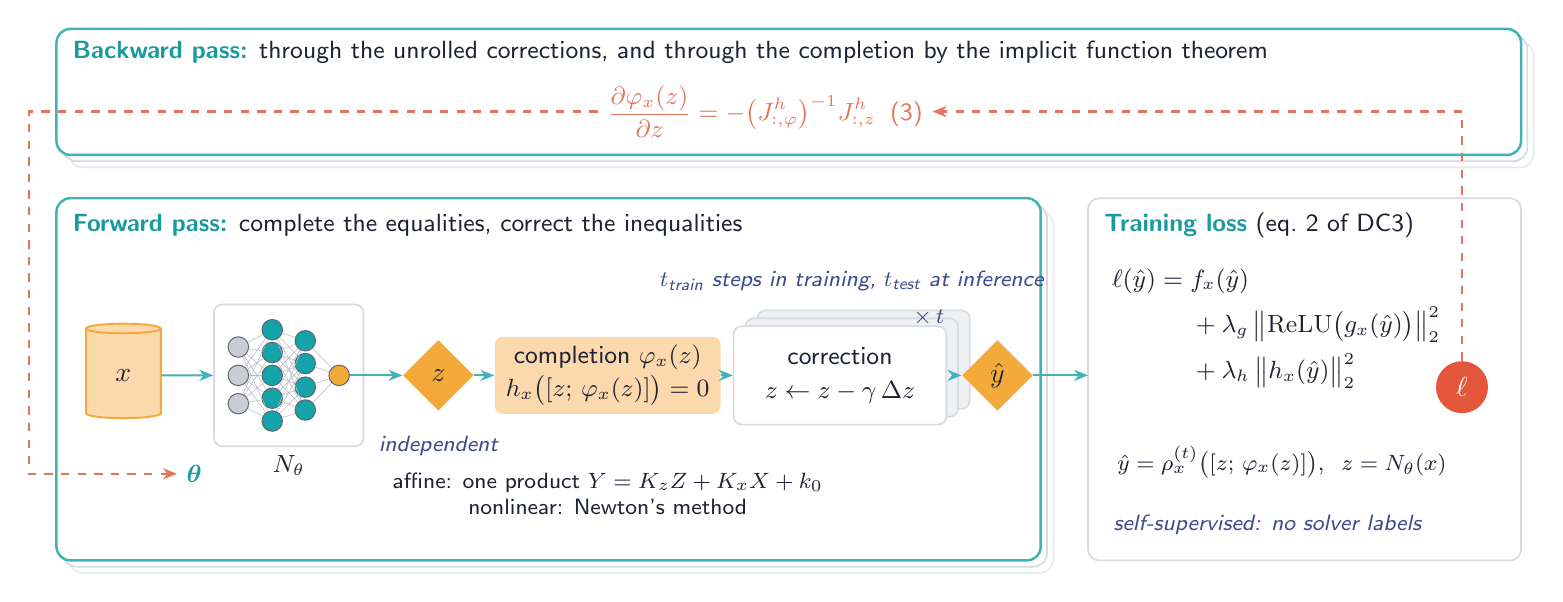
\begin{tikzpicture}
  % ---- backward band (top) ----
  \lane{0}{5.15}{18.6}{6.75}
  \node[title] at (0.2,6.45) {\textcolor{dTeal}{\bfseries Backward pass:} \textcolor{dInk}{through the unrolled corrections, and through the completion by the implicit function theorem}};
  \node[font=\small,text=dCoral] (ad) at (9.0,5.7) {\ift};

  % ---- forward (bottom left) ----
  \lane{0}{0}{12.5}{4.6}
  \node[title] at (0.2,4.25) {\textcolor{dTeal}{\bfseries Forward pass:} \textcolor{dInk}{complete the equalities, correct the inequalities}};
  \node[store] (x) at (0.85,2.35) {$x$};
  \net{2.95,2.35}{px}{0}
  \node[font=\small] at (2.95,1.2) {$N_\theta$};
  \node[font=\small\bfseries,text=dTeal] (th) at (1.75,1.1) {$\bm\theta$};
  \draw[fwd] (x.east) -- (pxsheet.west);
  \node[dia] (z) at (4.85,2.35) {$z$};
  \node[note] at (4.85,1.45) {independent};
  \draw[fwd] (pxout.east) -- (z.west);
  \node[chip,fill=dPeach,align=center,font=\small] (cp) at (7.0,2.35) {\complete};
  \draw[fwd] (z.east) -- (cp.west);
  \node[font=\footnotesize,align=center] at (7.0,0.85) {affine: one product $Y=K_zZ+K_xX+k_0$\\nonlinear: Newton's method};
  \unrolled{9.95,2.35}
  \draw[fwd] (cp.east) -- (corr.west);
  \node[note,align=center] at (10.1,3.55) {$t_{\text{train}}$ steps in training, $t_{\text{test}}$ at inference};
  \node[dia] (yh) at (11.95,2.35) {$\hat y$};
  \draw[fwd] (11.45,2.35) -- (yh.west);

  % ---- loss (bottom right) ----
  \cardbox{13.1}{0}{18.6}{4.6}
  \node[title] at (13.3,4.25) {\textcolor{dTeal}{\bfseries Training loss} (eq.\ 2 of DC3)};
  \node[anchor=north west,font=\small,inner sep=0pt] at (13.4,3.75) {\softloss};
  \node[font=\footnotesize,anchor=west] at (13.35,1.25) {$\hat y=\rho_x^{(t)}\big([z;\,\varphi_x(z)]\big),\;\; z=N_\theta(x)$};
  \node[note,anchor=west] at (13.3,0.45) {self-supervised: no solver labels};
  \draw[fwd] (yh.east) -- (13.1,2.35);
  \node[lnode] (l) at (17.85,2.2) {$\ell$};
  \draw[dual] (l.north) -- (l.north |- ad.east) -- (ad.east);
  \draw[dual] (ad.west) -| (-0.35,1.1) -- (th.west);
\end{tikzpicture}
\fi
\end{document}
